Pre-text Invariant Representation Learning (PIRL) \cite{misra2020self} is a SSL method that uses contrastive learning like CMC, but the intention of the author is to train a model which learn a representation of the input images that is invariant with respect to image transformations.
\begin{figure}[H]
	\centering
	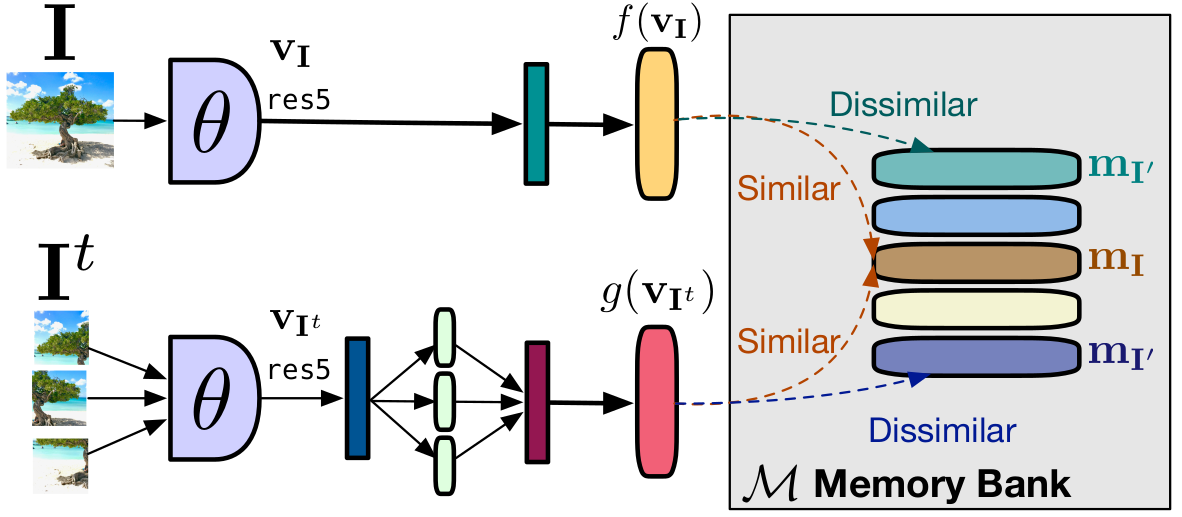
\includegraphics[width=8cm]{./images/pirl_scheme.png}
	\caption{Scheme that shows how PIRL works}
	\label{fig:pirl_scheme}
\end{figure}
\noindent Given a dataset $\mathcal{D} = \{I_1, \dots ,I_{|D|}\}$ where $I_n \in \mathbb{R}^{H\times W\times3}$ and set of transformation $\mathcal{T}$, the goal of PIRL is to train a convolutional neural network $\phi_\theta(\cdot)$ that constructs image representations $v_I = \phi_\theta(I)$ which are invariant to image transformations in $\mathcal{T}$. In order to do so $\phi_\theta$ is trained to minimize the following loss function:
\[ \ell_{inv}(\theta;\mathcal{D}) = \mathbb{E}_{t \sim p(\mathcal{T})}\Bigg[ \frac{1}{|D|} \sum_{I \in \mathcal{D}} L(v_I, v_{I^t}) \Bigg] \]
where $L(\cdot, \cdot)$ measures the similarity between two image representations. Minimization of this loss encourages the network $\phi_\theta(\cdot)$ to produce the same representation for the image $I$ as the transformed counter part $I^t$, so to make the representation invariant with respect to transformation $t$. $L(\cdot, \cdot)$ is defined as a contrastive loss:
\[h(v_I, v_{I^t}) = \frac{ \exp\Big(s(v_I, v_{I^t})/\tau \Big)}{ \exp\Big(s(v_I, v_{I^t})/\tau\Big) + \sum_{I^\prime \in \mathcal{D}_N}\exp\Big(s(v_I, v_{I^\prime})/\tau\Big)}\]
where $\mathcal{D}_N \subseteq \mathcal{D} \setminus \{I\}$ is a set of negative samples and $s(\cdot, \cdot)$ is a similarity function. Actually to compute the similarity we do not compute the features $v$ directly but we apply different heads. Specifically we use $f(\cdot)$ for $v_I$ and $g(\cdot)$ for $v_{I^t}$. So the actual loss is:
\[L_{\text{NCE}}(I, I^t) = -\log\big(h(f(v_I), g(v_{I^t}))\big) - \sum_{I^\prime \in \mathcal{D}_N} \log\big(1 - h(g(v^t_I), f(v_{I^\prime}))\big) \]
which encourages the representation of image $I$ to be similar to the one of its transformed counterpart $I^t$, while also encouraging it to be dissimilar to the representation of other images $I^\prime$.

To address this problem of finding many negative samples during the training the authors decided to use a memory bank $\mathcal{M}$ that contains the feature representation $m_I$ of image $I \in \mathcal{D}$. $m_I$ is an exponential moving average of the feature representation $f(v_I)$ that were computed in the prior epochs. In this way we can replace in th loss definition the negative samples $f(v^\prime_I)$ by their memory bank representation $m_{I^\prime}$, while keeping the batch size small. All the representation that are stored in the memory bank are all computed on the original images, $I$, without the transformation $t$. An issue of $L_{\text{NCE}}$ is that it does not compare the representation of the original image $I$ with the representation of the negative samples $I^\prime$, and this is fixed by using the following loss instead:
\[ L(I,I^t) = \lambda L_{\text{NCE}}(m_I, g(v_{I^t})) + (1-\lambda)L_{\text{NCE}}(m_I, f(v_I)) \]
where the first term is the one we had before and the second term encourages the representation of $f(v_I)$ to be similar to its memory bank representation $m_I$ and it also encourages the representation of $f(v_I)$ and $f(v_{I^\prime})$ to be dissimilar. 
